%! Author = kucera-lukas
%! Date = 4/13/22

\section{Steganografie}\label{sec:steganografie}

\subsection{Definice}\label{subsec:definice}
Steganografie je vědní disciplína (podobor kryptografie) zabývající se utajením
komunikace prostřednictvím ukrytí zprávy.
Zpráva je ukryta tak, aby si pozorovatel neuvědomil,
že komunikace vůbec probíhá.\cite{wiki:steganografie}

\subsection{Implementace}\label{subsec:implementace}
Uzivateli

\subsection{Zakodovani}\label{subsec:zakodovani-dat}
Na adrese \url{https://stegoer.netlify.app/encode} muze uzivatel nahrat svuj
obrazek a zakodovat do nej informaci.

\begin{subsubsection}{Textovy editor}\label{subsubsec:textovy-editor}
V horni casti stranky se nazachazi textovy editor.
Do nej uzivatel zada data, ktera maji byt skryta v obrazku.
Editor umoznuje mnoho moznosti pro formatovani textu.

\begin{figure}
    \centering
    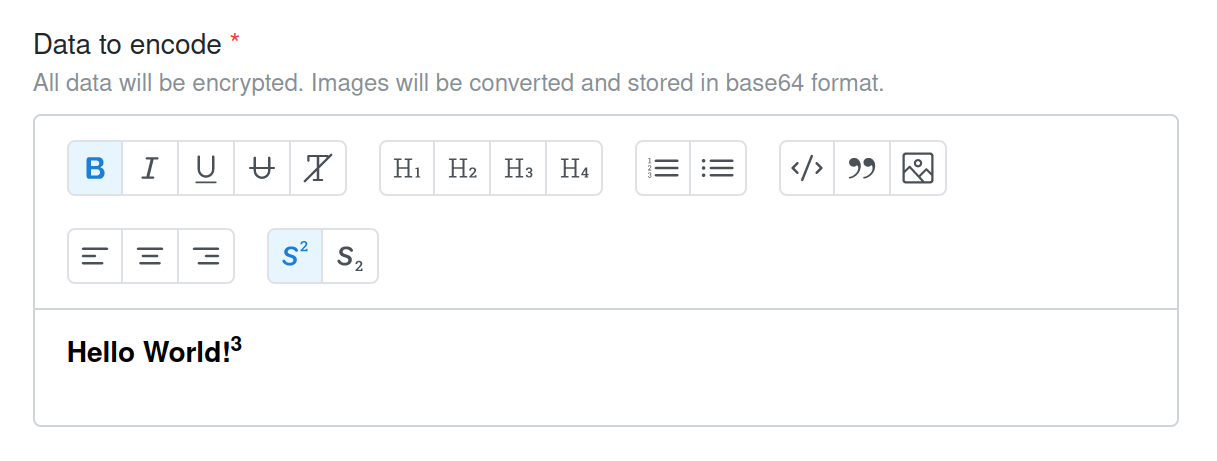
\includegraphics[scale=0.5]{assets/images/encode-editor}
    \caption{Editor textu pro data k zakodovani}\label{fig:editor-textu}
\end{figure}

\end{subsubsection}

\begin{subsubsection}{Konfigurace}\label{subsubsec:enc-konfigurace}

Konfigurace je dostupna pouze pro prihlasenye uzivatele.

V sekci \texttt{Advanced Configuration} je dostupne nastaveni parametru
pro zakodovani.

\begin{enumerate}
    \item Vlastni klic pro zasifrovani dat.
    \item Pocet nejmene vyznamnych bitu, ktere maji byt pouzity.
    \item Urceni jake barevne slozky maji byt zmeneny.
    \item Zda-li maji byt data rozpostrena po obrazku rovnomerne.
\end{enumerate}

\end{subsubsection}

\begin{figure}
    \centering
    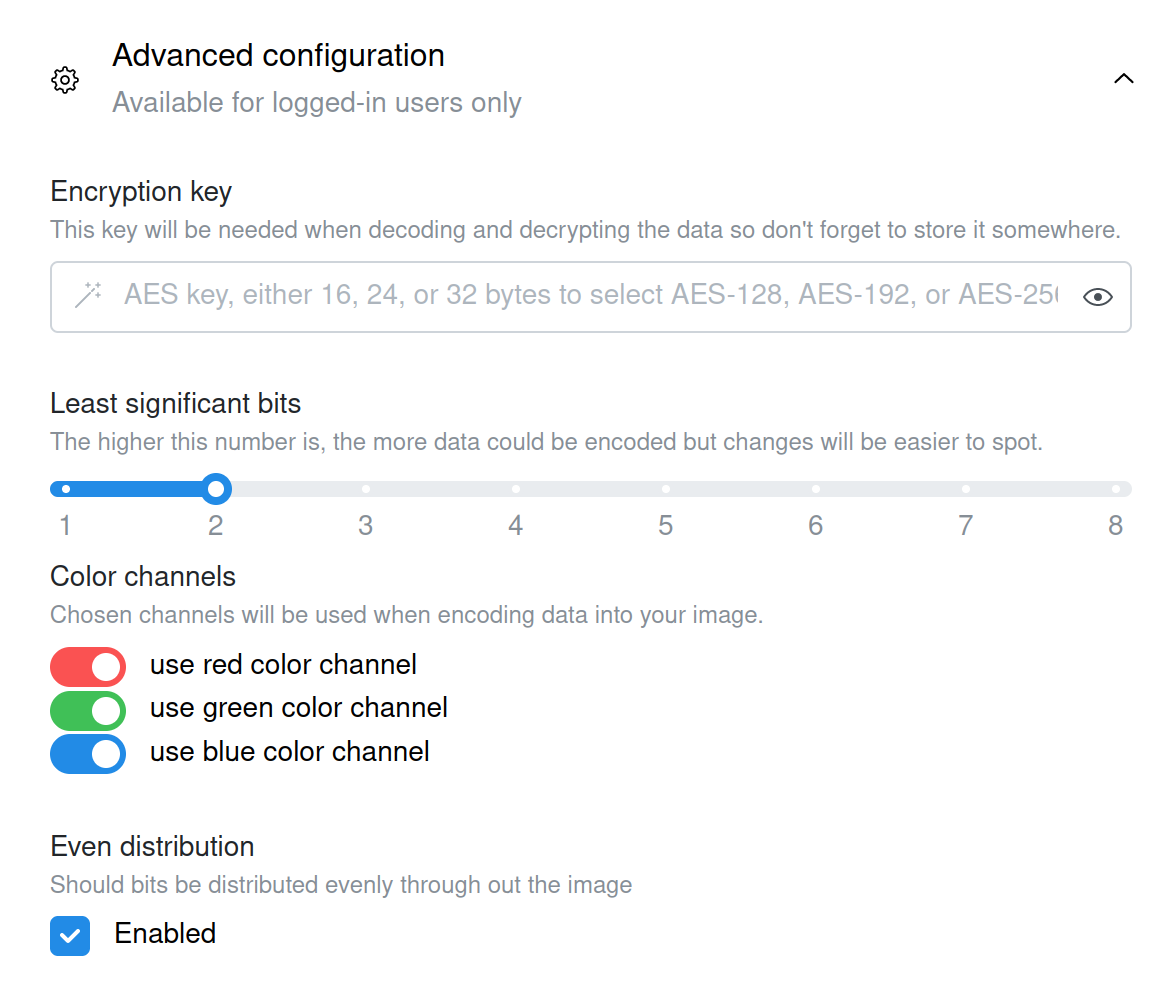
\includegraphics[scale=0.5]{assets/images/encode-configuration}
    \caption{Konfigurace zakodovani}\label{fig:konfigurace-zakodovani}
\end{figure}

\begin{subsubsection}{Nahrani obrazku}\label{subsubsec:enc-nahrani-obrazku}

Na strance nalezneme pole do ktereho lze nahrat obrazek.
Do nej budou informace zakodovany.

\end{subsubsection}

\begin{subsubsection}{Potvrzeni}\label{subsubsec:enc-potvrzeni}

Po stisknuti tlacitka \texttt{Encode} probehne kontrola vlozenych hodnot.
Pokud je nejaky problem nalezen aplikace uzivatele upozorni.
Dale aplikace posle pozadavek s informaci, konfiguraci a
obrazkem na server.
Nasledne server zpravu zasifruje rozdeli na jednotlive bity a zapise do obrazku.
Pokud vse probehne v poradku client dostane zpet odpoved s timto upravenym
obrazkem.
Uzivateli se pak nabidne moznost si obrazek stahnout.

\end{subsubsection}

\subsection{Dekodovani}\label{subsec:dekodovani-dat}
Na adrese \url{https://stegoer.netlify.app/decode} muze uzivatel nahrat svuj
obrazek a dekodovat z nej data, ktera tam v minulosti zakodoval.

\begin{subsubsection}{Konfigurace}\label{subsubsec:dec-konfigurace}

V sekci \texttt{Advanced Configuration}, ktera je opet dostupna pouze
prihlasenym uzivatelum, je mozne specifikovat vlastni klic, ktery ma byt pouzit
k odsifrovani zpravy.

\end{subsubsection}

\begin{subsubsection}{Nahrani obrazku}\label{subsubsec:dec-nahrani-obrazku}

Na strance opet nalezneme pole do ktereho lze nahrat obrazek.
Z tohotu obrazku se aplikace pokusi zakodovanou informaci dekodovat.

\end{subsubsection}

\begin{subsubsection}{Potvrzeni}\label{subsubsec:dec-potvrzeni}

Po stisknuti tlacitka \texttt{Decode} probehne kontrola vlozenych hodnot.
Pokud je vse v poradku aplikace posle pozadavek s obrazkem a konfiguraci na
server.
Nasledne server obrazek zpracuje a pokusi se zakodovanou informaci odsifrovat.
Pokud vse probehne v poradku client dostane zpet odpoved s odsifrovanou
informaci.
Na konci stranky se pak tato informace zobrazi.
Aplikace take informaci uzivateli zkopiruje do schranky, aby s ni mohl dale
pracovat.

\end{subsubsection}
